%*****************************************************************************************
%*********************************** First Chapter ***************************************
%*****************************************************************************************

\chapter{Motivation}  %Title of the First Chapter

\ifpdf
    \graphicspath{{Chapter1/Figs/Raster/}{Chapter2/Figs/PDF/}{Chapter2/Figs/}}
\else
    \graphicspath{{Chapter1/Figs/Vector/}{Chapter2/Figs/}}
\fi

Initially, this project was intended to be focused on skin detection and feature recognition for the potential application of hand tracking and posture prediction. However, it was quickly noticed that many authors were sticking to the RGB space, which suffers from disadvantages due to changes in lighting affecting the results. It was also noted that there seemed to be some significant disagreement over the methodology behind using a skin model~\cite{Shin2002a}~\cite{Sigal2000a}~\cite{Skarbek1994}~\cite{Soriano2000a}~\cite{Terrillon1999a}~\cite{Vezhnevets2003}~\cite{Brown2001a}. It appears that the reason many authors avoided luminosity-oriented color spaces was down to the computational intensity of performing the transform, the loss of information, and what seems like a rather perplexing issue to do with white-out, black-out and camera calibration. After reading over the literature, it was decided that two of these three issues were soluble, and the third was worthy of investigation.

\section{Overview of Color Spaces}

For the purposes of this project, a color space dedicated to human skin is necessary. When it comes to pattern recognition, it is beneficial to reduce the number of channels which the algorithm must process, as well as reducing the information density in those channels. It is also hoped that, in an appropriate color space, it will be a simple matter to separate the characteristics associated with saturation of tissue with blood, which changes under mechanical stress from the unchanging pigmentation of the cells (\cite{Stamatas2004}). Color spaces --- when they are normally defined --- are a combination of rotations, scaling and translations, while some (e.g. HSV (\cite{Vezhnevets2003, Zarit1999a} )) also perform a coordinate transform. The color space defined for this project is unusual in that it uses a non-linear redistribution of the values. It should be noted that this is not a pixel-based classifier (\cite{Jones2002}). However, seeing as the color space contains both the statistical information and the skin color information, it can be interpreted in a probabilistic way.

For the sake of comparison, the following four color spaces --- all of which have been used for skin detection (\cite{Vezhnevets2003,Zarit1999a,Yang1997a,Brand2000a,Sigal2000a,Chai2000a,Phung2002a}) --- have been evaluated for the purposes of this project.

\subsection{LAB}\label{sec:LAB}

The LAB color space's perceptual uniformity makes it well-suited for skin detection, as the human eye can perceive practically any change in its values (\cite{Vezhnevets2003,Poynton1997}). However, the Gaussian distribution of the skin is not positioned on the axis, which makes applying the statistics troublesome.

\subsection{RGB}\label{sec:RGB}

The RGB color space, while widely used, is perhaps the most ill-suited color space for skin detection, as it can't make a distinction between chrominance and luminance, as discussed by ~\cite{Vezhnevets2003,Brand2000a}. That said, its ubiquity in cameras --- which are designed to capture images which, to us, appear to be an accurate representation of physical reality despite the opposite being true --- makes it a necessary color space to work in. The advantage to using it is simply the fact that it is a straightforward, raw output from the camera.

\subsection{HSV}\label{sec:HSV}

Unlike RGB, the HSV color space makes a clear distinction between the chrominance (the "Hue" and "Saturation" channels) and the luminance (the "Value" channel), storing them separately (\cite{Vezhnevets2003,Sigal2000a}). This makes HSV a popular choice for skin segmentation, but it's difficult to control any information loss during the transform due to its non-linearity (\cite{Poynton1997}).

\subsection{YCbCr}\label{sec:YCbCr}

This color space bears similarities to the LAB and HSV spaces in that it explicitly separates the chrominance and the luminance. The luminosity (or "luma") channel "Y" is a weighted sum of the RGB values (\cite{Poynton1997,Phung2002a}), while the chrominance channels "Cb" and "Cr" contain the color difference between Y and the red and blue components of RGB, respectively (\cite{Vezhnevets2003}). Also like LAB, it is not oriented such that the Gaussian distribution is situated along the axis. In fact, there is little distinction between the two spaces aside from the orientation in the chromatic portion of the space.

The main issue with using these color spaces is the lack of control over information flow upon transformation and the clear mathematical statement of the transformation in terms of rotation, scaling and translation. Therefore, the construction of a new color space is necessary.

\section{Physiology Study}\label{sec:PhysiologyStudy}

The image captured by a CCD camera is designed to fool the human eye. In physical reality, light reaching the sensor spans full spectral range. In the human eye --- and in the camera --- the diversity of chromatic information is lost by representing the spectrum as a combination of three chromatic Gaussians, as can be seen in Figure~\ref{fig:spectrum}.

\begin{figure}[h!]
  \centering
    \includegraphics[width=\textwidth]{Chapter2/Figs/spectrum.eps}
    \caption{Human eye representation of the color spectrum.}  \label{fig:spectrum}
\end{figure}

Human skin is made up of two layers, each with its own optical properties: the surface layer --- the "epidermis" --- and the "dermis," the vascular structure underneath in which the blood vessels, lymphatic vessels and other such fibroblast structures can be found (~\cite{Stamatas2004}). The molecules which make up these layers make an important contribution to skin color. The most significant of these are melanin --- which is found in the epidermis --- and oxy-hemoglobin and deoxy-hemoglobin --- both of which reside in the dermis. Melanin is the main spectral absorber in the epidermis and the greatest contributor to the visual perception of surface skin color; it features a monotonic increase toward short wavelengths on its spectral absorption curve in the visible, approaching linear in the region 600-750 nm (~\cite{Stamatas2004,Kollias1995,Zonios2001}). Oxy-hemoglobin and deoxy-hemoglobin are actually different states of the same molecule --- hemoglobin --- which is found in the dermal blood supply. The molecule's chromophoric state is dependent upon whether it is delivering oxygen molecules to the tissues; it exists as oxy-hemoglobin if it is delivering oxygen and deoxy-hemoglobin if it isn't. The redness of skin in the areas where hemoglobin is found is due to the molecule's absorption of incident light (~\cite{Kollias1995}). It should be noted that each form of hemoglobin has its own characteristic absorption profile; oxy-hemoglobin's maxima on the absorption curve can be found at 415, 540 and 577 nm, whereas deoxy-hemoglobin's are located at 430 and 555 nm.

Seeing as the chromophores' absorption characteristics are expressed as wavelengths, it should be possible to turn a wavelength into a point in a color space. The absorption spectra is a complete description of the material. As such, it can be used to show what the material would look like under any lighting condition. The white light spectrum as perceived by the human eye can be represented using RGB Gaussian waveforms by turning the absorption spectra into a scattering spectra and representing it in terms of the RGB Gaussians. Through the use of an additive process based on Grassman's law, which states that, if the sample color is a combination of two monochromatic colors, then the value found by the observer for each monochromatic base color from the sample color will be the sum of each sample base color of the two monochromatic colors observed separately, we can find points in the R, G and B channels in the RGB color space for the three chromaphores (~\cite{MIHAI2007}).

The equivalent RGB points for the colors of the absorption peaks can be calculated as follows:

\begin{equation}
\begin{array}{cc}
 \{0.6\, -0.0136667 (\lambda -380),0,0.02 (\lambda -380)+0.39\} & \lambda \geq 380.\land \lambda \leq 410. \\
 \{0.19\, -0.00633333 (\lambda -410),0,1\} & \lambda \geq 410.\land \lambda \leq 440. \\
 \left\{0,\frac{\lambda -490}{50}+1,1\right\} & \lambda \geq 440.\land \lambda \leq 490. \\
 \left\{0,1,\frac{510-\lambda }{20}\right\} & \lambda \geq 490.\land \lambda \leq 510. \\
 \left\{\frac{\lambda -580}{70}+1,1,0\right\} & \lambda \geq 510.\land \lambda \leq 580. \\
 \left\{1,\frac{640-\lambda }{60},0\right\} & \lambda \geq 580.\land \lambda \leq 640. \\
 \{1,0,0\} & \lambda \geq 640.\land \lambda \leq 700. \\
 \{0.008125 (780-\lambda )+0.35,0,0\} & \lambda \geq 700.\land \lambda \leq 780. \\
\end{array}
 \\
\end{equation}

If the respective color is shined on a molecule with these properties, it will absorb them. To convert this into a scattering spectrum, spectrum of the incident light must be taken, subtracting the amount that is absorbed. Assuming a uniform line, the process is not unlike flipping the waveform on its Y axis.

\begin{figure}[h!]
  \centering
    \includegraphics[width=0.45\textwidth]{Chapter2/Figs/absOxyHemo.eps}
    
\includegraphics[width=0.45\textwidth]{Chapter2/Figs/absDeoxyHemo.eps}
    \includegraphics[width=0.45\textwidth]{Chapter2/Figs/absMelanin.eps}
    \caption{Oxy-hemoglobin, deoxy-hemoglobin and melanin absorption characteristics.}  \label{fig:abs}
\end{figure}

The scattering spectra needs to be represented in a three-function Gaussian basis. We will take the maximum values of these and make a quick transform of the scattering spectra, giving a color value for the molecules and their relative positions in the space. The scattering spectra are presented in Figure~\ref{fig:scat}.

\begin{figure}[h!]
  \centering
    \includegraphics[width=0.45\textwidth]{Chapter2/Figs/scatOxyHemo.eps}
    \includegraphics[width=0.45\textwidth]{Chapter2/Figs/scatDeoxyHemo.eps}
    
\includegraphics[width=0.45\textwidth]{Chapter2/Figs/scatMelanin.eps}
    \caption{Oxy-hemoglobin, deoxy-hemoglobin and melanin scattering spectra.}  \label{fig:scat}
\end{figure}

Finally, we perform a color matching operation based on the CIE 1931 standard observer piecewise function to complete the transformation.

\begin{figure}[h!]
  \centering
    \includegraphics[width=\textwidth]{Chapter2/Figs/colorBasis.eps}
    \caption{Final skin chromophore positions.}  \label{fig:colorBasis}
\end{figure}

We have a function for the light source, but we will make the crude assumption of an equal amount of all wavelengths. This is sufficient for the purposes of this project.

%********************************** %First Section  **************************************
%\section{Motivation} %Section - 1.1 





%********************************** %Second Section  *************************************
%\section{Overview of Color Spaces} %Section - 1.2


%********************************** % Third Section  *************************************
%\section{Where does it come from?}  %Section - 1.3 
%\label{section1.3}


